\documentclass{boi2014}

\usepackage{enumitem}
\usepackage{wrapfig}
\usepackage{mathtools}
\usepackage{tikz}

\renewcommand{\DayNum}{1}
\renewcommand{\TaskCode}{coprobber}
\renewcommand{\TaskName}{Politseinik ja röövel}

\renewcommand{\labelitemii}{$\circ$}
\newcommand{\constant}[1]{{\tt #1}}

\begin{document}
    \begin{wrapfigure}[8]{r}{6cm}
        \vspace{-24pt}
		\includegraphics[width=6cm]{\TaskCode.jpeg}
	\end{wrapfigure}

    Bytemore'i linnas on kuritegevus tõusnud kõigi aegade kõrgeimale tasemele. 
    Muude kuritegude hulgas pannakse igapäevaselt toime röövimisi. 
    Kui kuritegu on sooritatud, peab üksik patrullpolitseinik röövli kinni püüdma, joostes läbi kitsaste tänavate, mis ühendavad tänavanurki. 
    Kahjuks pääsevad röövlid enamasti minema, sest nad tunnevad linna oluliselt paremini kui politseinikud.

    Bytemore City Police Department (BCPD) korraldas nõupidamise kuritegevuse vähendamiseks. 
    Üks vastuvõetud otsustest on kasutada röövlite tabamiseks arvutite abi. 
    Selleks on BCPD loonud linna täpse kaardi, aga nüüd vajatakse tarkvara jälitamisstrateegiate leidmiseks.

    Jälitamisstrateegia, kus üks politseinik jälitab üht röövlit, saab modelleerida järgmiselt:
    \begin{enumerate}
        \item Politseinik valib, millisel tänavanurgal ta patrullib.
        \item Röövel valib, millisel tänavanurgal ta röövib (teades ette, kus politseinik on). Sellest hetkest alates saame eeldada, et nii politseinik kui ka röövel teavad alati, kus vastane asub.
        \item Politseiniku käik võib olla kas liikumine naabernurgale (sellisele tänavanurgale, millele praeguselt nurgalt, läbides ühe tänava) või ootamine (jäädes paigale).
        \item Röövel liigub oma käigul alati mõnele naabernurgale. Erinevalt politseinikest ei suuda röövlid paigal püsida, nende instinkt sunnib neid alati jooksma.
        \item Politseinik ja röövel teevad kordamööda käike (politseinik alustab), kuni juhtub üks kahest tulemusest:
        \begin{enumerate}
            \item Seis kordab mõnda eelnevat (seis on defineeritud kombinatsioonina mõlema isiku asukohast ning sellest, kelle käigukord on). Kordus tähendab, et röövel suudab politseinikku lõputult vältida, nii et ta pääseb põgenema.
            \item Politseinik ja röövel kohtuvad samal nurgal (pärast ükskõik kumma käiku). Sel juhul saab politseinik röövli kätte.
        \end{enumerate}
    \end{enumerate}

    \Task
    Kirjutada programm, mis otsustab linnaplaani põhjal, kas röövli tabamine on võimalik, ja kui on, siis püüab röövli kinni, tehes politseiniku eest käike.

    Programm peab eeldama, et röövel teeb optimaalseid käike.

    \Implementation
    Realiseerida kaks funktsiooni:
    \begin{itemize}
        \item \method{start(N, A)}, mis saab järgmised parameetrid:
            \begin{itemize}
                \item $N$ --- tänavanurkade arv (nurgad on märgistatud arvudega 
                    $0$ kuni $N-1$);
                \item $A$ --- kahemõõtmeline massiiv, mis kirjeldab tänavaid: iga $0 \le i, j \le N-1$ korral
                    $$
                        A[i, j] \text{ on }
                        \begin{dcases*}
                            \texttt{false}, & kui $i$ ja $j$ ei ole tänavaga ühendatud
                                \\
                            \texttt{true}, & kui $i$ ja $j$ on tänavaga ühendatud
                        \end{dcases*}
                    $$
                    Kõik tänavad on kahesuunalised (s.t iga $i$ ja $j$ korral $A[i, j] = A[j, i]$)
                    ja ükski tänav ei ühenda tänavanurka iseendaga
                    (s.t iga $i$ korral $A[i, i]$ on
                    \texttt{false}).  Saab ka eeldada,
                    et igalt tänavanurgalt on mööda tänavaid liikudes alati võimalik jõuda 
                    igale teisele nurgale.
            \end{itemize}

        Kui röövlit on võimalik parameetritega kirjeldatud kaardil tabada,
        siis funktsioon \method{start} peab tagastama tänavanurga numbri,
        millel politseinik otsustab patrullida.
        Vastasel korral tagastada $-1$.

        \item Funktsioon \method{nextMove(R)} saab parameetrina tänavanurga
            numbri $R$, millel röövel parajasti asub,
            ja peab tagastama selle nurga numbri, millel politseinik pärast
            oma järgmist käiku asub.
    \end{itemize}

    	Funktsiooni \method{start} kutsutakse välja täpselt üks kord,
    enne \method{nextMove} väljakutseid. Kui \method{start} tagastab
    $-1$, siis \method{nextMove} välja ei kutsuta. Vastasel korral kutsutakse
    \method{nextMove} välja kuni jälitamine lõpeb.
    Täpsemalt, programm lõpetab töö, kui juhtub üks järgmistest
    asjaoludest:
    \begin{itemize}
        \item \method{nextMove} tagastab ebakorrektse käigu;
        \item tekib korduv seis;
        \item röövel saadakse kätte.
    \end{itemize}

    \Example
    \begin{wrapfigure}[4]{r}{2cm}
        \vspace{-0.5cm}
        \centering
        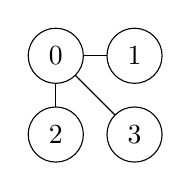
\begin{tikzpicture}
        \draw (0,1) -- (0,0);
        \draw (0,1) -- (1,0);
        \draw (0,1) -- (1,1);
        \foreach \x in {0,1} \foreach \y in {0,1}
            \draw (\x,\y) node[circle,draw,fill=white,inner sep=0,minimum size=0.7cm] {\pgfmathparse{int(2-2*\y+\x)}\pgfmathresult};
        \end{tikzpicture}
    \end{wrapfigure}
    Vaatame parempoolsel joonisel toodud näidet. Antud juhul võib
    politseinik alustada suvaliselt nurgalt. Kui ta alustab 
    nurgalt 0, võib ta oma esimesel käigul oodata ja röövel jookseb ise tema juurde.
    Teise võimalusena võib ta alustada suvaliselt teiselt nurgalt, oodata, kuni röövel 
    jookseb nurka 0, ning siis ise ka sinna minna.
    
    Näidissessioon näeks välja järgmine:

    \begin{tabular}{|l|c|}
        \hline
            {\bf Funktsiooni väljakutse} & {\bf Tagastab} \\
        \hline
            \method{start(4, [[0, 1, 1, 1], [1, 0, 0, 0], [1, 0, 0, 0], [1, 0, 0, 0]])} &
            \constant{3} \\
        \hline
            \method{nextMove(1)} & \constant{3} \\
        \hline
            \method{nextMove(0)} & \constant{0} \\
        \hline
    \end{tabular}

    Märkus: Lühiduse mõttes tähistab \method{start} funktsiooni väljakutses \constant{0} 
    \constant{false} ning \constant{1} tähistab \constant{true}.

    \Scoring
    Maksimaalsete punktide saamiseks peab lahendus:
    \begin{enumerate}
    	\item Õigesti leidma, kas politseinikul on võimalik röövel kätte saada;
	\item Politseiniku eest käike tehes röövli edukalt kinni püüdma.
    \end{enumerate}
    
    Lahendused, mis täidavad ainult esimese nõude, saavad alamülesannetes 3 ja 4
    30\% vastava alamülesande punktidest. 

    \begin{description}
        \item[Alamülesanne 1 (16 punkti):] $2 \le N \le 500$. Iga tänavanurkade paari vahel on täpselt üks võimalik tee.
        \item[Alamülesanne 2 (14 punkti):] $2 \le N \le 500$. Tänavanurkade ja tänavate kaart 
        moodustab ruudustiku. Ruudustikul on vähemalt
        kaks rida ja veergu ning tänavanurgad on märgistatud alltoodud joonisel
        näidatud viisil.
        \begin{figure}[h!]
           \centering
           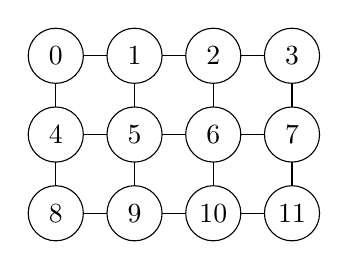
\begin{tikzpicture}
            \draw (0,0) grid (3,2);
            \foreach \x in {0,1,2,3} \foreach \y in {0,1,2}
                \draw (\x,\y) node[circle,draw,fill=white,inner sep=0,minimum size=0.7cm] {\pgfmathparse{int(8-4*\y+\x)}\pgfmathresult};
           \end{tikzpicture}
        \end{figure}
        \item[Alamülesanne 3 (30 punkti):] $2 \le N \le 100$.
        \item[Alamülesanne 4 (40 punkti):] $2 \le N \le 500$.
    \end{description}

    \Constraints
    
    \begin{description}
        \item[Ajapiirang:] 1 s.
        \item[Mälupiirang:] 256 MB.
    \end{description}

    \Experimentation
    Näidishindaja teie arvutis loeb andmeid standardsisendist.
    Sisendi esimesel real on täisarv $N$ --- tänavanurkade arv.
    Järgmised $N$ rida sisaldavad naabrusmaatriksi $A$ ridu.
    Igal neist ridadest on $N$ arvu väärtustega 0 või 1.
    Maatriks peab olema sümmeetriline ja selle peadiagonaali väärtused
    peavad olema nullid.

    Järgmine rida sisaldab arvu 1, kui politseinik saab röövli kätte ja
    0 vastasel juhul.

    Lõpuks, kui politseinik saab röövli kätte, järgnevad $N$ rida, mis kirjeldavad
    röövli strateegiat.  Igaüks neist ridadest sisaldab 
    $N+1$ täisarvu 0 ja $N-1$ vahel.  Väärtus reas $r$ ja veerus $c$,
    kus $c < N$, vastab seisule, kus röövli kord on käia, politseinik
    on nurgal $r$ ja röövel on nurgal $c$.
    Väärtus ise tähistab tänavanurka, millele röövel liigub.  Peadiagonaali
    väärtusi ignoreeritakse, kuna nad vastavad seisudele, kus röövel ja politseinik
    on juba samal nurgal.  Rea $r$ viimane arv tähistab 
    röövli stardinurka, mis vastab politseiniku stardinurgale $r$.

    Järgnevalt on toodud näidissisend näidishindajale, mis tähistab kolme tänavanurka, mis 
    on omavahel ühendatud:

    \begin{center}
        \begin{tabular}{p{4cm}}
            {\tt
                3 \newline
                0 1 1 \newline
                1 0 1 \newline
                1 1 0 \newline
                1 \newline
                0 2 1 2 \newline
                2 0 0 2 \newline
                1 0 0 1 \newline
            }
        \end{tabular}
    \end{center}

    Järgnevalt on toodud näidissisend, mis vastab eelpool toodud näitele:

    \begin{center}
        \begin{tabular}{p{4cm}}
            {\tt
                4 \newline
                0 1 1 1 \newline
                1 0 0 0 \newline
                1 0 0 0 \newline
                1 0 0 0 \newline
                1 \newline
                0 0 0 0 1 \newline
                2 0 0 0 2 \newline
                3 0 0 0 3 \newline
                1 0 0 0 1 \newline
            }
        \end{tabular}
    \end{center}
\end{document}
